\documentclass{article}

% Language setting
% Replace `english' with e.g. `spanish' to change the document language
\usepackage[english]{babel}

% Set page size and margins
% Replace `letterpaper' with`a4paper' for UK/EU standard size
\usepackage[letterpaper,top=2cm,bottom=2cm,left=3cm,right=3cm,marginparwidth=1.75cm]{geometry}

% Useful packages
\usepackage{amsmath}
\usepackage{graphicx}
\usepackage[colorlinks=true, allcolors=blue]{hyperref}

\title{Elliptic Curves and the Nagell-Lutz theorem:\\a guided reinvention}
\author{Samuel Dauncey}

\begin{document}
\maketitle

\begin{abstract}
    
"Number theory has an annoying habit: the field produces, without effort, innumerable problems which have a sweet, innocent air about them, tempting flowers; and yet... number theory swarms with bugs, waiting to bite the tempted flower-lovers who, once bitten, are inspired to excesses of effort!" - Barry Mazur
\end{abstract}

\section{Introduction and Motivation}

Suppose one wanted to find all solutions to the innocent - looking polynomial equation:\\

$3 X^3 +  2 X Y^2 + 2 Y^3 = Z^3$ \quad For integers $X$, $Y$ and $Z$. \\

 One may realise that, given a solution; say $(X, Y, Z) = (1, 2, 3)$, one can see that we can generate infintely many more solutions $(X, Y, Z) = (2, 4, 6), \; (3, 6, 9), \; \dots \; (n, 2n, 3n) \; \dots $. This property of our equation is special, it is called \emph{homogeneity} and stems from the fact that if we sum up the powers of $X$, $Y$ and $Z$ in each of the terms of our equation, we get the same integer (in this case, three). \\
 
 Finding solutions to homogeneous equations is of special importance to number theorists, examples including the Fermat equation $X^m + Y^m = Z^m$. \\
 
 In essence, we can think of each of these infinite sets of solutions as all part of the same solution, and we can see that, if we view our solutions as coordinates in $R^3$, each one of our infinite sets of solutions can be viewed as a line going through the origin and and a point with integer coordinates. Dividing our original equation by $Z$, we can see that our problem is equivalent to finding the rational solutions to the equation:\\
 
 $3x^3 + 2xy + y^3 = 1$\\
 
With rational solution $(x, y) = (\frac{m}{n}, \frac{p}{q})$ being converted into $(X, Y, Z) = (m, p, nq)$ and integer solution $(X, Y, Z)$ being converted into $(\frac{X}{Z}, \frac{Y}{Z})$. However, note that this conversion isn't well-defined when $Z = 0$, so we still have to consider the integer solutions to $3 X^3 +  2 X Y^2 + 2 Y^3 = 0$. However; as this is also a homogeneous polynomial equation, we can repeat our process, this time by dividing by $Y$ to see we want to find solutions to: \\

$3 x^3 + 2 x + 2 = 0$ \quad for rational $x$ and $X^3 = 0$ for integer $X$\\

Hence, we can see that there is a one-to-one correspondence between the "lines" of integer solutions to $3 X^3 +  2 X Y^2 + 2 Y^3 = Z^3$ and rational solutions to  $3x^3 + 2xy + y^3 = 1$, \quad $3 x^3 + 2 x + 2 = 0$, and $X^3 = 0$. Thinking back to our visualisation of our solutions to our integer equation as lines, we can see that our first division resembles looking at the intersection of the plane $Z = 1$ and our solution lines, and the fact that we could recursively apply this procedure is a hint that the \emph{projective space} we are working in has some kind of recursive structure.

Now, we can trivially solve $X^3 = 0 $ to see that $X = 0$ is the only solution (corresponding to the solution $(X, Y, Z) = (0, 0, 0)$). Slightly more difficult is the rational solutions to $3x^3 + 2 x + 2 = 0$; Gauss's Lemma tells us that any solution in it's lowest terms $x = \frac{m}{n}$ must have $m$ dividing $2$ and $n$ dividing $3$, however we can see that the only candidates this leaves, $x = +-\frac{2}{3}$ do not solve the equation; so we have no solutions of the form $(X, Y, 0)$ with non-zero $Y$. Hence, we can see that the only thing stopping us from solving our starting problem is finding the rational solutions to  $3x^3 + 2xy + y^3 = 1$; unfortunately, this turns out to be alot harder. \\

These solutions form an \emph{algebraic curve} when visualised in the $x,y-$plane, and through analysing this curve geometrically we will be able to get some description of our solution.\\

Note that, given two points $(x_1, y_1)$ and $(x_2, y_2)$ on a degree-3 algebraic curve defined by $f(x, y) = 0$, we can find a third point $(x_3, y_3)$ on the curve by projecting a line $\alpha x + \beta y + \gamma = 0$ through them and looking at the intersection with the curve (in general*). On top of this, when we solve these simultaneous equations by eliminating one variable we get two cubics for the $x$ and $y$ coordinates, $a_3 x^3 + a_2 x^2 + a_1 x + a_0 = 0$ , \quad $b_3 y^3 + b_2 y^2 + b_1 y + b_0 = 0$. We know that the sums $x_1 + x_2 + x_3 = -\frac{a_2}{a_3}$ and $y_1 + y_2 + y_3 = -\frac{b_2}{b_3}$ are satisfied; so if $x_1$, $x_2$ and our coefficients are in some field $F$, $x_3$ must also be in $F$; and likewise for our $y$ coordinates, this means that, given a pair of rational solutions we can get another solution by projecting a line.

* the case where $a_3$ or $b_3$ are zero corresponds to the case where our line meets our curve asymptotically, or "at infinity", and we will see more about this when we go into projective geometry.
\\ 

The first theorem we will prove is the Mordell-Wiel theorem, which tells us that we can take a finite set of rational points on our curve and, by projecting lines through them, can get every other rational point on our curve.\\

The Nagell-Lutz theorem gives us a set of criteria which we can use to build an algorithm for all of the points that form "cycles" through our operation of addition.\\


 
 
 
 
 
 

\section{Some examples to get started}

\subsection{How to create Sections and Subsections}

Simply use the section and subsection commands, as in this example document! With Overleaf, all the formatting and numbering is handled automatically according to the template you've chosen. If you're using Rich Text mode, you can also create new section and subsections via the buttons in the editor toolbar.

\subsection{How to include Figures}

First you have to upload the image file from your computer using the upload link in the file-tree menu. Then use the includegraphics command to include it in your document. Use the figure environment and the caption command to add a number and a caption to your figure. See the code for Figure \ref{fig:frog} in this section for an example.

Note that your figure will automatically be placed in the most appropriate place for it, given the surrounding text and taking into account other figures or tables that may be close by. You can find out more about adding images to your documents in this help article on \href{https://www.overleaf.com/learn/how-to/Including_images_on_Overleaf}{including images on Overleaf}.
\newpage
\begin{figure}
\centering
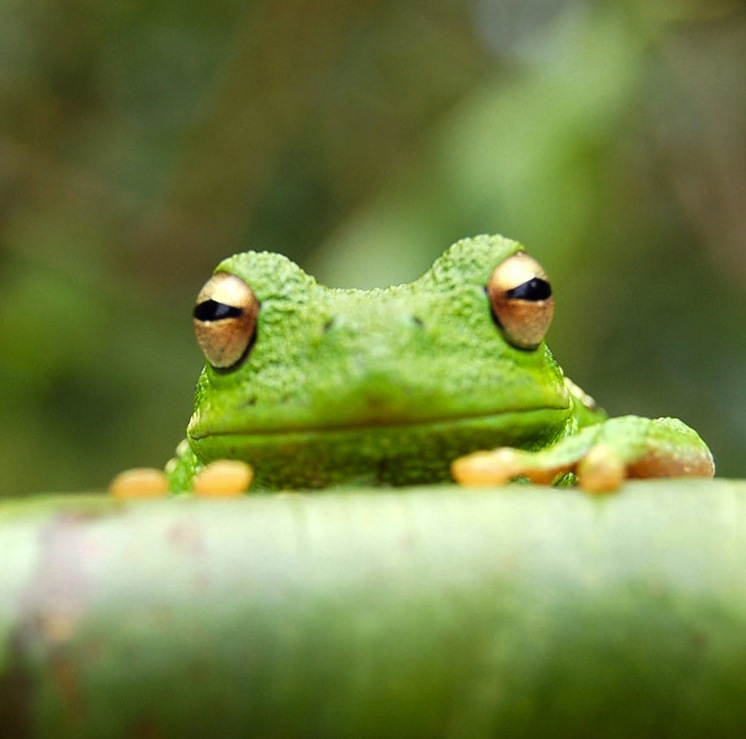
\includegraphics[width=0.3\textwidth]{frog.jpg}
\caption{\label{fig:frog}This frog was uploaded via the file-tree menu.}
\end{figure}

\subsection{How to add Tables}

Use the table and tabular environments for basic tables --- see Table~\ref{tab:widgets}, for example. For more information, please see this help article on \href{https://www.overleaf.com/learn/latex/tables}{tables}. 

\begin{table}
\centering
\begin{tabular}{l|r}
Item & Quantity \\\hline
Widgets & 42 \\
Gadgets & 13
\end{tabular}
\caption{\label{tab:widgets}An example table.}
\end{table}

\subsection{How to add Comments and Track Changes}

Comments can be added to your project by highlighting some text and clicking ``Add comment'' in the top right of the editor pane. To view existing comments, click on the Review menu in the toolbar above. To reply to a comment, click on the Reply button in the lower right corner of the comment. You can close the Review pane by clicking its name on the toolbar when you're done reviewing for the time being.

Track changes are available on all our \href{https://www.overleaf.com/user/subscription/plans}{premium plans}, and can be toggled on or off using the option at the top of the Review pane. Track changes allow you to keep track of every change made to the document, along with the person making the change. 

\subsection{How to add Lists}

You can make lists with automatic numbering \dots

\begin{enumerate}
\item Like this,
\item and like this.
\end{enumerate}
\dots or bullet points \dots
\begin{itemize}
\item Like this,
\item and like this.
\end{itemize}

\subsection{How to write Mathematics}

\LaTeX{} is great at typesetting mathematics. Let $X_1, X_2, \ldots, X_n$ be a sequence of independent and identically distributed random variables with $\text{E}[X_i] = \mu$ and $\text{Var}[X_i] = \sigma^2 < \infty$, and let
\[S_n = \frac{X_1 + X_2 + \cdots + X_n}{n}
      = \frac{1}{n}\sum_{i}^{n} X_i\]
denote their mean. Then as $n$ approaches infinity, the random variables $\sqrt{n}(S_n - \mu)$ converge in distribution to a normal $\mathcal{N}(0, \sigma^2)$.


\subsection{How to change the margins and paper size}

Usually the template you're using will have the page margins and paper size set correctly for that use-case. For example, if you're using a journal article template provided by the journal publisher, that template will be formatted according to their requirements. In these cases, it's best not to alter the margins directly.

If however you're using a more general template, such as this one, and would like to alter the margins, a common way to do so is via the geometry package. You can find the geometry package loaded in the preamble at the top of this example file, and if you'd like to learn more about how to adjust the settings, please visit this help article on \href{https://www.overleaf.com/learn/latex/page_size_and_margins}{page size and margins}.

\subsection{How to change the document language and spell check settings}

Overleaf supports many different languages, including multiple different languages within one document. 

To configure the document language, simply edit the option provided to the babel package in the preamble at the top of this example project. To learn more about the different options, please visit this help article on \href{https://www.overleaf.com/learn/latex/International_language_support}{international language support}.

To change the spell check language, simply open the Overleaf menu at the top left of the editor window, scroll down to the spell check setting, and adjust accordingly.

\subsection{How to add Citations and a References List}

You can simply upload a \verb|.bib| file containing your BibTeX entries, created with a tool such as JabRef. You can then cite entries from it, like this: \cite{greenwade93}. Just remember to specify a bibliography style, as well as the filename of the \verb|.bib|. You can find a \href{https://www.overleaf.com/help/97-how-to-include-a-bibliography-using-bibtex}{video tutorial here} to learn more about BibTeX.

If you have an \href{https://www.overleaf.com/user/subscription/plans}{upgraded account}, you can also import your Mendeley or Zotero library directly as a \verb|.bib| file, via the upload menu in the file-tree.

\subsection{Good luck!}

We hope you find Overleaf useful, and do take a look at our \href{https://www.overleaf.com/learn}{help library} for more tutorials and user guides! Please also let us know if you have any feedback using the Contact Us link at the bottom of the Overleaf menu --- or use the contact form at \url{https://www.overleaf.com/contact}.

\bibliographystyle{alpha}
\bibliography{sample}

\end{document}